\begin{name}
	{Biên soạn \& Phản biện: Nhóm 1}
	{Sở GD \& ĐT Phú Thọ (Lần 2)}
\end{name}
\Opensolutionfile{ansbook}[ans/ansb\currfilebase]
\caulc
\Opensolutionfile{ans}[ans/ans\currfilebase-Phan-I]
\begin{ex}%[Dự án KYMP81-VN-MT-15]%[2-KS-20-SoPhuTho-L2-2026,TV037]%[1D5N1-4]
	Lâm trường Tam Đảo thống kê đường kính thân gỗ của $60$ cây xoan đào được cho ở bảng sau:
	\begin{center}
		\begin{tabular}{|c|c|c|c|c|c|}
			\hline 
			Đường kính (cm) & $[20; 22)$ &$[22; 24)$ &$[24; 26)$ &$[26; 28)$ &$[28; 30)$ \\
			\hline 
			Tần số & $5$ & $20$ & $18$ & $7$ & $10$ \\
			\hline
		\end{tabular}
	\end{center}
	Nhóm chứa mốt của mẫu số liệu đã cho là
	\choice
		{$[20;22)$}
		{$[28;30)$}
		{$[24;26)$}
		{\True $[22;24)$}
	\loigiai{
		Do tần số lớn nhất là $20$ nên nhóm chứa mốt của mẫu số liệu đã cho là $[22;24)$.
	}
\end{ex}

\begin{ex}%[Dự án 5EL79Y-VN-MT-15]%[2-KS-20-SoPhuTho-L2-2026,TV037]%[0D0H2-5]
	Một hộp có $5$ viên bi màu đỏ và $7$ viên bi màu xanh. Lấy ngẫu nhiên $2$ viên bi từ hộp đó. Xác suất để lấy được $2$ viên bi màu đỏ bằng
	\choice
		{\True $\dfrac{5}{33}$}
		{$\dfrac{5}{22}$}
		{$\dfrac{2}{33}$}
		{$\dfrac{7}{22}$}
	\loigiai{
		Ta có $n(\Omega) = \mathrm{C}_{12}^2 = 66$. \\
		Gọi $A$ là biến cố: \lq\lq Lấy được $2$ viên bi màu đỏ\rq\rq. \\
		Suy ra $n(A) = \mathrm{C}_5^2 = 10$. \\
		Xác suất để lấy được $2$ viên bi màu đỏ là
		\[\mathrm{P}(A) = \dfrac{n(A)}{n(\Omega)} = \dfrac{10}{66} = \dfrac{5}{33}.\]
	}
\end{ex}

\begin{ex}%[Dự án 1JVYIG-VN-MT-15]%[2-KS-20-SoPhuTho-L2-2026,TV037]%[2H5H2-3]
	Trong không gian $Oxyz$, đường thẳng đi qua hai điểm $A(1;2;3)$, $B(5;4;-1)$ có phương trình chính tắc là
	\choice
		{$\dfrac{x+1}{2}=\dfrac{y+2}{1}=\dfrac{z+3}{-2}$}
		{$\dfrac{x-1}{2}=\dfrac{y-2}{1}=\dfrac{z-3}{2}$}
		{$\dfrac{x+5}{-2}=\dfrac{y+4}{-1}=\dfrac{z-1}{2}$}
		{\True $\dfrac{x-5}{2}=\dfrac{y-4}{1}=\dfrac{z+1}{-2}$}
	\loigiai{
		Ta có $\overrightarrow{AB} = (4;2;-4)$. \\
		Đường thẳng $AB$ đi qua điểm $B(5;4;-1)$ và nhận $\overrightarrow{u} = \dfrac{1}{2}\overrightarrow{AB} = (2;1;-2)$ làm một vectơ chỉ phương nên có phương trình chính tắc là
		\[\dfrac{x-5}{2} = \dfrac{y-4}{1} = \dfrac{z+1}{-2}.\]
	}
\end{ex}

\begin{ex}%[Dự án 1AMN7Z-VN-MT-15]%[2-KS-20-SoPhuTho-L2-2026,TV037]%[2D4H2-1]
	Cho $\displaystyle\int\limits_2^5 f(x) \mathrm{\,d}x=2$ và $\displaystyle\int\limits_2^5 g(x) \mathrm{\,d}x=5$. Giá trị của tích phân $\displaystyle\int\limits_2^5 \big[f(x)-2 g(x)\big] \mathrm{d}x$ bằng
	\choice
		{\True $-8$}
		{$12$}
		{$1$}
		{$-3$}
	\loigiai{
		Ta có $\displaystyle\int\limits_2^5 \big[f(x)-2 g(x)\big] \mathrm{d}x = \displaystyle\int\limits_2^5 f(x) \mathrm{\,d}x - 2\displaystyle\int\limits_2^5 g(x) \mathrm{\,d}x = 2 - 2\cdot 5 = -8$.
	}
\end{ex}

\begin{ex}%[Dự án 21T9QA-VN-MT-15]%[2-KS-20-SoPhuTho-L2-2026,TV037]%[0D7H3-2]
	Biết phương trình $\sqrt{2x^2+x+3}=1-x$ có hai nghiệm phân biệt $x_1$; $x_2$. Tổng $x_1+x_2$ bằng
	\choice
		{\True $-3$}
		{$-1$}
		{$2$}
		{$-2$}
	\loigiai{
		Ta có 
		\allowdisplaybreaks
		\begin{eqnarray*}
			&& \sqrt{2x^2+x+3}=1-x \\
			&\Rightarrow& 2x^2 + x + 3 = 1 - 2x + x^2 \\
			&\Rightarrow& x^2 + 3x + 2 = 0 \\
			&\Rightarrow& \hoac{&x=-1\\&x=-2.}
		\end{eqnarray*}
		Thử lại, ta thấy $x=-1$, $x=-2$ đều thỏa mãn. \\
		Vậy $x_1+x_2 = -1 + (-2) = -3$.
	}
\end{ex}

\begin{ex}%[Dự án 31JA8B-VN-MT-15]%[2-KS-20-SoPhuTho-L2-2026,TV037]%[1D2H2-4]
	Cho cấp số cộng $(u_n)$ có $u_1=-2$ và công sai $d=3$. Giá trị của $u_{10}$ bằng
	\choice
		{$-2\cdot 3^9$}
		{$-29$}
		{\True $25$}
		{$28$}
	\loigiai{
		Ta có $u_{10} = u_1 + 9d = -2 + 9\cdot 3 = 25$.
	}
\end{ex}

\begin{ex}%[Dự án 5IU0G7-VN-MT-15]%[2-KS-20-SoPhuTho-L2-2026,TV002]%[1D7H2-1]
	Đạo hàm của hàm số $f(x) = \sin x + \cos 3x$ là
	\choice
		{$f'(x) = -\cos x + 3\sin 3x$}
		{\True $f'(x) = \cos x - 3\sin 3x$}
		{$f'(x) = \cos x + 3\sin 3x$}
		{$f'(x) = -\cos x + \sin 3x$}
	\loigiai{
		Ta có $f'(x) = (\sin x)' + \big(\cos 3x \big)' = \cos x - 3\sin 3x$.
	}
\end{ex}

\begin{ex}%[Dự án 1HV8I0-VN-MT-15]%[2-KS-20-SoPhuTho-L2-2026,TV002]%[1D6H4-3]
	Tập nghiệm của bất phương trình $\log_{\tfrac{1}{3}} (2x - 1) > -2$ là
	\choice
		{\True $\left(\dfrac{1}{2}; 5\right)$}
		{$\left(\dfrac{1}{2}; +\infty\right)$}
		{$(5; +\infty)$}
		{$(-\infty; 5)$}
	\loigiai{
		Điều kiện xác định $2x - 1 > 0 \Leftrightarrow x > \dfrac{1}{2}$.\\
		Bất phương trình đã cho trở thành
		\[ 2x - 1 < \left(\dfrac{1}{3}\right)^{-2} \Leftrightarrow 2x - 1 < 9 \Leftrightarrow 2x < 10 \Leftrightarrow x < 5. \]
		So với điều kiện xác định, ta được tập nghiệm của bất phương trình là $S = \left(\dfrac{1}{2}; 5\right)$.
	}
\end{ex}

\begin{ex}%[Dự án 3CU0VA-VN-MT-15]%[2-KS-20-SoPhuTho-L2-2026,TV002]%[2D1H2-1]
	Cho hàm số $y = f(x)$ có đạo hàm là $f'(x) = (x-1)(x-2)^2(x+3)$, $\forall x \in \mathbb{R}$. Số điểm cực trị của hàm số đã cho là
	\choice
		{\True $2$}
		{$3$}
		{$1$}
		{$0$}
	\loigiai{
		Ta có $f'(x) = 0 \Leftrightarrow \hoac{&x = 1 &&\text{(nghiệm bội lẻ)} \\ &x = 2 &&\text{(nghiệm bội chẵn)} \\ &x = -3 &&\text{(nghiệm bội lẻ).}}$\\
		Vì phương trình $f'(x)=0$ có $2$ nghiệm bội lẻ nên số điểm cực trị của hàm số đã cho là $2$.
	}
\end{ex}

\begin{ex}%[Dự án 5H4247-VN-MT-15]%[2-KS-20-SoPhuTho-L2-2026,TV002]%[2D1H3-1]
	Giá trị lớn nhất của hàm số $f(x) = \dfrac{2x+3}{x-1}$ trên đoạn $[2; 5]$ bằng
	\choice
		{$\dfrac{13}{4}$}
		{$5$}
		{\True $7$}
		{$2$}
	\loigiai{
		Xét hàm số $f(x) = \dfrac{2x+3}{x-1}$ xác định và liên tục trên đoạn $[2; 5]$.\\
		Ta có $f'(x) = \dfrac{-5}{(x-1)^2} < 0$, $\forall x \in [2; 5]$.\\
		Suy ra hàm số $f(x)$ nghịch biến trên đoạn $[2; 5]$.\\
		Vậy giá trị lớn nhất của hàm số trên đoạn $[2; 5]$ là $\max\limits_{[2; 5]} f(x) = f(2) = \dfrac{2 \cdot 2 + 3}{2 - 1} = 7$.
	}
\end{ex}

\begin{ex}%[Dự án 6BXUOH-VN-MT-15]%[2-KS-20-SoPhuTho-L2-2026,TV002]%[1D1N5-3]
	Tập nghiệm của phương trình $\sin x = 0$ là
	\choice
		{$S = \left\{\dfrac{\pi}{2} + k\pi,\, k \in \mathbb{Z}\right\}$}
		{\True $S = \big\{k\pi,\, k \in \mathbb{Z}\big\}$}
		{$S = \big\{k2\pi,\, k \in \mathbb{Z}\big\}$}
		{$S = \big\{\pi + k2\pi,\, k \in \mathbb{Z}\big\}$}
	\loigiai{
		Ta có $\sin x = 0 \Leftrightarrow x = k\pi$, $k \in \mathbb{Z}$.\\
		Vậy tập nghiệm của phương trình là $S = \{k\pi,\, k \in \mathbb{Z}\}$.
	}
\end{ex}

\begin{ex}%[Dự án 4KYSN4-VN-MT-15]%[2-KS-20-SoPhuTho-L2-2026,TV002]%[2H2H1-2]
	Cho hình hộp chữ nhật $ABCD.A'B'C'D'$ có $AB = 2$, $AD = 3$, $AA' = 6$. Độ dài vectơ $\overrightarrow{AB} + \overrightarrow{AD} + \overrightarrow{AA'}$ bằng
	\choice
		{\True $7$}
		{$7\sqrt{3}$}
		{$11\sqrt{3}$}
		{$11$}
	\loigiai{
		\begin{center}
			\begin{tikzpicture}[scale=1, font=\footnotesize, line join=round, line cap=round, >=stealth]
    %hidden: VM005
				\def\a{3}
				\def\b{2}
				\def\h{3.5}
				\path 	(0:0) coordinate (A)
					++(0:\a) coordinate (D)
					++(-130:\b) coordinate (C)
					($(A)+(C)-(D)$) coordinate (B)
					($(A)+(90:\h)$) coordinate (A')
					($(B)+(90:\h)$) coordinate (B')
					($(C)+(90:\h)$) coordinate (C')
					($(D)+(90:\h)$) coordinate (D');
				\draw[dashed] 	(B)--(A)--(D)	(A)--(A');
				\draw (C)--(C') (D)--(D') 	(B)--(B') (C)--(C') (B)--(C)--(D) (A')--(B')--(C')--(D')--cycle;
				\foreach \x/\g in {A/180,B/180,C/0,D/0,A'/180,B'/180,C'/0,D'/0}
				\fill (\x) circle (1pt)
					($(\g:4mm)+(\x)$) node {$\x$};	
    \node at (0,0){\href{4KYSN4}{\tiny \phantom{4KYSN4}}};
			\end{tikzpicture}
		\end{center}
		Theo quy tắc hình hộp, ta có $\overrightarrow{AB} + \overrightarrow{AD} + \overrightarrow{AA'} = \overrightarrow{AC'}$.\\
		Ta có $AC' = \sqrt{AB^2 + AD^2 + AA'^2} = \sqrt{2^2 + 3^2 + 6^2} = \sqrt{49} = 7$.\\
		Vậy $\left| \overrightarrow{AB} + \overrightarrow{AD} + \overrightarrow{AA'} \right| = \left| \overrightarrow{AC'} \right| = 7$.
	}
\end{ex}

\Closesolutionfile{ans}
\cauds
\Opensolutionfile{ans}[ans/ans\currfilebase-Phan-II]
\begin{ex}%[Dự án 1QLZ1K-VN-MT-15]%[2-KS-20-SoPhuTho-L2-2026,VM007]%[2H5H3-3]
	Trong không gian $Oxyz$, cho $A(0;1;1)$, $B(1;0;-3)$, $C(-1;-2;-3)$ và mặt cầu $(S)$ có phương trình $x^2 + y^2 + z^2 - 2x + 2z - 2 = 0$.
	\choiceTF
		{\True $\overrightarrow{AB} = (1; -1; -4)$}
		{Điểm $G(a;b;c)$ là trọng tâm của tam giác $\triangle ABC$ thì $a+b+c = 2$}
		{Mặt phẳng $(ABC)$ có phương trình $2x - 2y + z - 1 = 0$}
		{\True Mặt phẳng $(ABC)$ cắt mặt cầu $(S)$ theo một đường tròn có bán kính bằng $\dfrac{4\sqrt{2}}{3}$}	
	\loigiai{
		\begin{itemchoice}
			\itemch Tọa độ vectơ $\overrightarrow{AB}=(1-0;0-1;-3-1)=(1;-1;-4)$.
			\itemch Ta có $G$ là trọng tâm của tam giác $ABC$ nên suy ra
			\[
			\heva{&a=\dfrac{0+1-1}{3}\\&b=\dfrac{1+0-2}{3}\\&c=\dfrac{1-3-3}{3}}
			\Leftrightarrow \heva{&a=0\\&b=-\dfrac{1}{3}\\&c=-\dfrac{5}{3}.}
			\]
			Suy ra $a+b+c=0-\dfrac{1}{3}-\dfrac{5}{3}=-2$.
			\itemch Tọa độ $\overrightarrow{AB}=(1;-1;-4)$, $\overrightarrow{AC}=(-1;-3;-4)$.\\
			Một vectơ pháp tuyến của $(ABC)$ là $\left[\overrightarrow{AB},\overrightarrow{AC}\right]=(-8;8;-4)$.\\
			Phương trình mặt phẳng $(ABC)$ là 
			\[
			-8(x-0)+8(y-1)-4(z-1)=0
			\Leftrightarrow 2x-2y+z+1=0.
			\]
			\itemch Mặt cầu $(S)$ có tâm $I(1;0;-1)$ và bán kính $R=2$.\\
			Khoảng cách từ tâm $I$ của mặt cầu $(S)$ đến mặt phẳng $(ABC)$ là 
			\[
			\mathrm{d}=\mathrm{\,d}\big(I,(ABC)\big)=\dfrac{|2\cdot 1-2\cdot 0-1+1|}{\sqrt{2^2+(-2)^2+1^2}}=\dfrac{2}{3}.
			\]
			\begin{center}
				\begin{tikzpicture}[scale=1, font=\footnotesize, line join=round, line cap=round, >=stealth]
    %hidden: VM005
					\def\r{1.5} \def\d{0.9}
					\path 
						(0,0) coordinate (O)
						($(O)+(\r,0)$) coordinate (A)
						($(O)+(0,\d)$) coordinate (I)
						;
					\coordinate (O) at (0,0);
					%\draw (O) ellipse (\r cm and 0.32cm);
					\draw[dashed] (A) arc (0:180:\r cm and 0.32cm);
					\draw (A) arc (0:-180:\r cm and 0.32cm); 
					\draw (I) let \p1=($(I)-(A)$) in circle ({veclen(\x1,\y1)});
					\draw[dashed] (I)--(O) node[midway,left]{$\mathrm{d}$}--(A)--cycle;
					\fill (I) circle(1pt) node[above]{$I$};
					\fill (O) circle(1pt) node[left]{$H$};				
    \node at (0,0){\href{1QLZ1K}{\tiny \phantom{1QLZ1K}}};
				\end{tikzpicture}
			\end{center}
			Suy ra mặt phẳng $(ABC)$ cắt mặt cầu $(S)$ theo một đường tròn có bán kính \[
			r=\sqrt{R^2-\mathrm{\,d}^2}=\sqrt{2^2-\left(\dfrac{2}{3}\right)^2}=\dfrac{4\sqrt{2}}{3}.
			\]
		\end{itemchoice}
	}
\end{ex}

\begin{ex}%[Dự án 5HRQ8R-VN-MT-15]%[2-KS-20-SoPhuTho-L2-2026,VM007]%[2D4H2-6]
	Một cây cà chua khi mới trồng có chiều cao $15$\,cm. Gọi $h(t)$ là chiều cao của cây cà chua tại thời điểm đúng $t$ tuần sau khi trồng (đơn vị: cm, $0 \leq t \leq 16$). Biết rằng tốc độ tăng chiều cao của cây cà chua đó được cho bởi hàm số $h'(t) = -0{,}02t^3 + 0{,}32t^2$ (đơn vị: cm/tuần).
	\choiceTF
		{Tại thời điểm đúng $t$ tuần sau khi trồng, chiều cao của cây cà chua là $h(t) = -\dfrac{t^4}{200} + \dfrac{32t^3}{300}$\,(cm)}
		{\True Tại thời điểm đúng $6$ tuần sau khi trồng, chiều cao của cây cà chua là $31{,}56$\,(cm)}
		{Tại thời điểm tốc độ tăng chiều cao của cây cà chua lớn nhất, cây cà chua cao hơn $80$\,(cm)}
		{\True Trong khoảng thời gian $10$ tuần đầu kể từ khi trồng, tốc độ tăng chiều cao trung bình của cây cà chua lớn hơn $5{,}6$\,(cm/tuần)}	
	\loigiai{
		\begin{itemchoice}
			\itemch Chiều cao của cây cà chua là một nguyên hàm của $h'(t)$. Suy ra 
			\[
			h(t)=\displaystyle\int h'(t) \mathrm{d}t
			=\displaystyle\int \left(-0{,}02t^3+0{,}32t^2\right) \mathrm{d}t
			=-0{,}02\cdot \dfrac{t^4}{4}+0{,}32\cdot \dfrac{t^3}{3}+C
			=-\dfrac{1}{200}t^4+\dfrac{32}{300}t^3+C.
			\]
			Cây cà chua khi mới trồng ($t=0$) có chiều cao $15$\,cm nên $h(0)=15\Leftrightarrow C=15$.\\
			Vậy tại thời điểm đúng $t$ tuần sau khi trồng, chiều cao của cây cà chua là 
			\[
			h(t)=-\dfrac{1}{200}t^4+\dfrac{8}{75}t^3+15\,\text{(cm)}.
			\]
			\itemch Tại thời điểm đúng $6$ tuần sau khi trồng, cây cà chua có chiều cao là 
			\[
			h(6)=-\dfrac{1}{200}\cdot 6^4+\dfrac{8}{75}\cdot 6^3+15
			=31{,}56\,\text{(cm)}.
			\]
			\itemch Đạo hàm $h''(t)=-0{,}06t^2+0{,}64t$.\\
			Xét phương trình $h''(t)=0\Leftrightarrow \hoac{&t=0\in [0;16]\\&t=\dfrac{32}{3}\in [0;16].}$\\
			Các giá trị $h'(0)=0$; $h'\left(\dfrac{32}{3}\right)=\dfrac{8\,192}{675}\approx 12{,}14$; $h'(16)=0$.\\
			Suy ra $\max\limits_{t\in [0;16]}h'(t)=h'\left(\dfrac{32}{3}\right)=\dfrac{8\,192}{675}$.\\
			Vậy cây cà chua có tốc độ tăng chiều cao lớn nhất khi $t=\dfrac{32}{3}$.\\
			Khi đó chiều cao của cây cà chua là $h\left(\dfrac{32}{3}\right)=79{,}73$.
			\itemch Tốc độ tăng chiều cao trung bình của cây cà chua trong $10$ tuần đầu kể từ khi trồng là
			\[
			h'_{\text{tb}}=\dfrac{1}{10-0}\displaystyle\int\limits_0^{10} h'(t)\mathrm{d}t
			=\dfrac{1}{10}\displaystyle\int\limits_0^{10} \left(-0{,}02t^3 + 0{,}32t^2\right)\mathrm{d}t
			=\dfrac{17}{3}\approx 5{,}67 \,\text{(cm/tuần)}.
			\]
		\end{itemchoice}
	}
\end{ex}

\begin{ex}%[Dự án 1EO66C-VN-MT-15]%[2-KS-20-SoPhuTho-L2-2026,VM027]%[2D6H2-4]
	Một công ty đấu thầu hai dự án. Xác suất trúng thầu dự án thứ nhất là $0{,}8$. Nếu trúng thầu dự án thứ nhất thì xác suất trúng thầu dự án thứ hai là $0{,}9$. Nếu không trúng thầu dự án thứ nhất thì xác suất trúng thầu dự án thứ hai là $0{,}2$.
	\choiceTF
		{\True Xác suất để công ty không trúng thầu dự án thứ nhất là $0{,}2$}
		{\True Xác suất để công ty trúng thầu cả hai dự án là $0{,}72$}
		{\True Xác suất để công ty trúng thầu dự án thứ hai là $0{,}76$}
		{Nếu công ty không trúng thầu dự án thứ hai thì xác suất trúng thầu dự án thứ nhất là $0{,}12$}
	\loigiai{
		Gọi $A_1$ là biến cố \lq\lq Công ty trúng thầu dự án thứ nhất\rq\rq.\\
		Gọi $A_2$ là biến cố \lq\lq Công ty trúng thầu dự án thứ hai\rq\rq.
		\begin{center}
			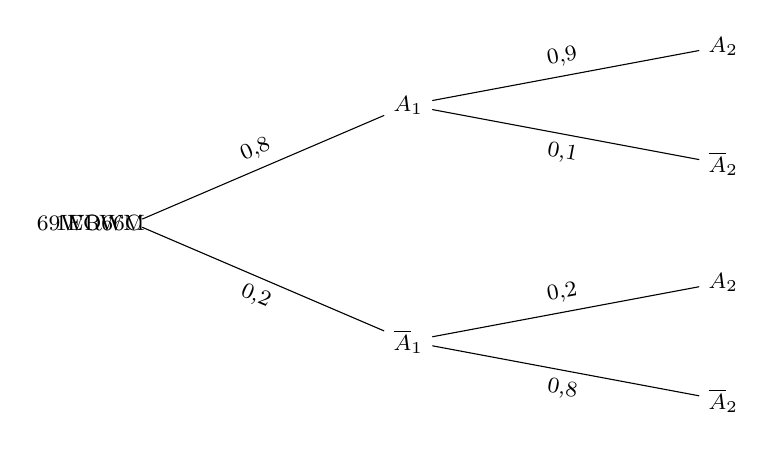
\begin{tikzpicture}[grow=right, sloped, level 1/.style={sibling distance=3cm, level distance=3.5cm}, level 2/.style={sibling distance=1.5cm, level distance=4cm}, scale=1, font=\footnotesize, line join=round, line cap=round, >=stealth]
    %hidden: VM005
				\node {}
				child {	node {$\overline{A}_1$}
				child {	node {$\overline{A}_2$}
				edge from parent node[below] {$0{,}8$}	}
				child {	node {$A_2$}
				edge from parent node[above] {$0{,}2$}	}
				edge from parent node[below] {$0{,}2$}	}
				child {	node {$A_1$}	child {	node {$\overline{A}_2$}
				edge from parent node[below] {$0{,}1$}}
				child {	node {$A_2$}
				edge from parent node[above] {$0{,}9$}}
				edge from parent node[above] {$0{,}8$}	};
				\node at (0,0){\href{69WRWM}{\tiny \phantom{69WRWM}}};
    \node at (0,0){\href{1EO66C}{\tiny \phantom{1EO66C}}};
			\end{tikzpicture}
		\end{center}
		\begin{itemchoice}
			\itemch Xác suất để công ty không trúng thầu dự án thứ nhất là 
			\[\mathrm{P}\left(\overline{A}_1\right)=1-\mathrm{P}(A_1) = 1 - 0{,}8 = 0{,}2.\]
			\itemch Xác suất để công ty trúng thầu cả hai dự án là
			\allowdisplaybreaks
			\begin{align*}
				\mathrm{P}(A_1 A_2) &= \mathrm{P}(A_1) \cdot \mathrm{P}(A_2 \mid A_1)\\
				&= 0{,}8 \cdot 0{,}9\\
				&= 0{,}72.
			\end{align*}
			\itemch Xác suất để công ty trúng thầu dự án thứ hai là
			\allowdisplaybreaks
			\begin{align*}
				\mathrm{P}( A_2) &= \mathrm{P}(A_1A_2) + \mathrm{P}\left(\overline{A}_1A_2\right)\\
				&= \mathrm{P}(A_1) \cdot \mathrm{P}(A_2 \mid A_1) + \mathrm{P}\left(\overline{A}_1\right) \cdot \mathrm{P}( A_2 \mid \overline{A}_1)\\
				&= 0{,}8 \cdot 0{,}9 + 0{,}2 \cdot 0{,}2\\
				&= 0{,}72 + 0{,}04\\
				&= 0{,}76.
			\end{align*}
			\itemch Xác suất trúng thầu dự án thứ nhất biết rằng công ty không trúng thầu dự án thứ hai là $\mathrm{P}( A_1 \mid \overline{A}_2)$.\\
			Ta có $\mathrm{P}(A_2 \mid A_1)= 0{,}9 \Rightarrow \mathrm{P}\left(\overline{A}_2 \mid A_1\right)=1-0{,}9=0{,}1$.\\
			Suy ra $\mathrm{P}\left(A_1\overline{A}_2\right) = \mathrm{P}(A_1) \cdot \mathrm{P}\left(\overline{A}_2 \mid A_1\right)= 0{,}8 \cdot 0{,}1 = 0{,}08$.\\
			Và xác suất để công ty không trúng thầu dự án thứ hai là \[\mathrm{P}\left(\overline{A}_2\right)= 1 - \mathrm{P}(A_2) = 1 - 0{,}76 = 0{,}24.\]
			Do đó $\mathrm{P}\left(A_1 \mid \overline{A}_2\right) = \dfrac{\mathrm{P}\left(A_1\overline{A}_2\right) }{\mathrm{P}\left(\overline{A}_2\right)} = \dfrac{0{,}08}{0{,}24} = \dfrac{1}{3} \approx 0{,}33$.
		\end{itemchoice}
	}
\end{ex}

\begin{ex}%[Dự án 1Q06NB-VN-MT-15]%[2-KS-20-SoPhuTho-L2-2026,VM027]%[2D1H4-1]
	Cho hàm số $y = \dfrac{x^2-3x+6}{x-1}$.
	\choiceTF
		{Hàm số nghịch biến trên khoảng $(-1;3)$}
		{\True Đường tiệm cận xiên của đồ thị hàm số là đường thẳng $y = ax + b$. Khi đó $a-2b = 5$}
		{\True Đường thẳng đi qua hai điểm cực trị của đồ thị hàm số có phương trình là $y = 2x-3$}
		{\True Gọi $A$, $B$ lần lượt là các điểm cực đại, cực tiểu của đồ thị hàm số và $O$ là gốc tọa độ. Diện tích tam giác $OAB$ bằng $6$}
	\loigiai{
		\begin{itemchoice}
			\itemch Tập xác định $\mathscr{D} = \mathbb{R} \setminus \{1\}$.\\
			Ta có $y = \dfrac{x^2-3x+6}{x-1}= x-2 + \dfrac{4}{x-1}$.\\
			Đạo hàm $y' = 1-\dfrac{4}{\left(x-1\right)^2} = \dfrac{x^2-2x-3}{\left(x-1\right)^2}$.\\
			Ta có $y' = 0 \Leftrightarrow x^2-2x-3 = 0 \Leftrightarrow \hoac{&x = -1\\&x = 3.}$\\
			Bảng biến thiên
			\begin{center}
				\begin{tikzpicture}
    %hidden: VM005
					\tkzTabInit[nocadre=true,lgt=1,espcl=2.5]
					{$x$/0.7, $y'$/0.7, $y$/2}
					{$-\infty$,$-1$, $1$,$3$, $+\infty$}
					% Dòng dấu đạo hàm
					\tkzTabLine{,+,0,-,d,-,0,+,}
					% Dòng giá trị hàm số
					\tkzTabVar{-/$-\infty$,+/ $-5$ ,-D+/ $-\infty$/$+\infty$ ,-/ $3$,+/$+\infty$}
    \node at (T11){\href{1Q06NB}{\tiny \phantom{1Q06NB}}};
				\end{tikzpicture}
			\end{center}
			Hàm số nghịch biến trên các khoảng $(-1;1)$ và $(1;3)$.\\
			Vậy phát biểu hàm số nghịch biến trên khoảng $(-1;3)$ là sai vì đồ thị bị gián đoạn tại $x = 1$.
			\itemch Ta có $\lim\limits_{x \to \pm\infty} \left[y-(x-2)\right] = \lim\limits_{x \to \pm\infty} \dfrac{4}{x-1} = 0$.\\
			Suy ra đồ thị hàm số có đường tiệm cận xiên là $y = x-2$.\\
			Do đó $a = 1$, $b = -2 \Rightarrow a-2b = 1-2(-2) = 5$.
			\itemch
			\textbf{Cách 1:} 
			Điểm cực đại của đồ thị hàm số là $A(-1; -5)$.\\
			Điểm cực tiểu của đồ thị hàm số là $B(3; 3)$.\\
			Đường thẳng $d$ đi qua hai điểm cực trị $A$ và $B$ nhận $\overrightarrow{AB} = (4; 8)$ làm vectơ chỉ phương.\\
			Suy ra $d$ có một vectơ pháp tuyến là $\overrightarrow{n} = (2; -1)$.\\			
			Phương trình tổng quát của đường thẳng $d$ đi qua $A(-1; -5)$ là
			\[ 2(x+1) - 1(y+5)=0 \Leftrightarrow 2x-y-3 = 0 \Leftrightarrow y = 2x-3. \]
			\textbf{Cách 2:}		
			Phương trình đường thẳng đi qua hai điểm cực trị của đồ thị hàm số phân thức bậc hai trên bậc nhất $y = \dfrac{u(x)}{v(x)}$ có dạng $y = \dfrac{u'(x)}{v'(x)}$.\\
			Áp dụng công thức, ta có phương trình đường thẳng đi qua hai điểm cực trị là
			\[y = \dfrac{\left(x^2-3x+6\right)'}{(x-1)'} = \dfrac{2x-3}{1} = 2x-3.\]
			\itemch Các điểm cực trị của đồ thị hàm số là $A(-1;-5)$ và $B(3; 3)$.\\
			Ta có $\mathrm{d}(O,AB)=\dfrac{|2\cdot 0-0-3|}{\sqrt{2^2+(-1)^2}}=\dfrac{3\sqrt{5}}{5}$ và $AB=\sqrt{4^2+8^2}=4\sqrt{5}$.\\
			Diện tích tam giác $OAB$ là
			\allowdisplaybreaks
			\begin{align*}
				S_{\triangle OAB} &= \dfrac{1}{2}\cdot \mathrm{d}(O,AB)\cdot AB\\
				&=\dfrac{1}{2}\cdot\dfrac{3\sqrt{5}}{5}\cdot 4\sqrt{5}\\
				&=6.
			\end{align*}
		\end{itemchoice}
	}
\end{ex}

\Closesolutionfile{ans}
\caukq
\Opensolutionfile{ans}[ans/ans\currfilebase-Phan-III]
\begin{ex}%[Dự án 6BV599-VN-MT-15]%[2-KS-20-SoPhuTho-L2-2026,VM008]%[0D7V2-7]
	Nếu một doanh nghiệp sản xuất $x$ sản phẩm trong một tháng ($x \in \mathbb{N}^*$, $1 \le x \le 5\,000$) thì doanh thu nhận được khi bán hết số sản phẩm đó là $F(x)=-0{,}03x^2+800x$ (nghìn đồng), trong khi chi phí sản xuất bình quân cho một sản phẩm là $G(x)=\dfrac{50\,000}{x}+450$ (nghìn đồng). Giả sử số sản phẩm sản xuất ra luôn được bán hết. Trong một tháng, doanh nghiệp đó cần sản xuất ít nhất bao nhiêu sản phẩm để lợi nhuận thu được lớn hơn $100$ triệu đồng?
	\par\shortans{$446$}
	\loigiai{
		Đổi $100$ triệu đồng $= 100\,000$ (nghìn đồng).\\
		Tổng chi phí sản xuất $x$ sản phẩm là
		\[C(x)=x \cdot G(x)=x \left( \dfrac{50\,000}{x}+450 \right)=50\,000+450x \text{ (nghìn đồng)}.\]
		Lợi nhuận của doanh nghiệp là
		\allowdisplaybreaks
		\begin{align*}
			L(x) &= F(x)-C(x) \\
			&= -0{,}03x^2+800x-(50\,000+450x) \\
			&= -0{,}03x^2+350x-50\,000 \text{ (nghìn đồng)}.
		\end{align*}
		Để lợi nhuận lớn hơn $100$ triệu đồng, ta có
		\allowdisplaybreaks
		\begin{eqnarray*}
			& &-0{,}03x^2+350x-50\,000 > 100\,000 \\
			&\Leftrightarrow& -0{,}03x^2+350x-150\,000 > 0\\
			&\Leftrightarrow& x_1 < x < x_2.
		\end{eqnarray*}
		Trong đó $x_1\approx 445{,}59$, $x_2 \approx 11\,221{,}08$.\\
		Do $x \in \mathbb{N}^*$ và $1 \le x \le 5\,000$, nên $x \in \{446; 447; \dots; 5\,000\}$.\\
		Vậy doanh nghiệp cần sản xuất ít nhất $446$ sản phẩm.
	}
\end{ex}

\begin{ex}%[Dự án 5I0FX9-VN-MT-15]%[2-KS-20-SoPhuTho-L2-2026,VM008]%[1H8V7-5]
	Cho hình lăng trụ $ABCD.A'B'C'D'$ có đáy $ABCD$ là hình thoi, số đo góc $\widehat{ABC}=60^\circ$. Biết rằng $C'A=C'B=C'C$. Góc giữa mặt phẳng $\left(BCC'B'\right)$ và mặt phẳng $(ABC)$ bằng $45^\circ$. Khoảng cách giữa hai đường thẳng $AA'$ và $BC$ bằng $6\sqrt{3}$. Thể tích khối lăng trụ đã cho bằng $a\sqrt{2}$, giá trị của $a$ bằng bao nhiêu?
	\par\shortans{$864$}
	\loigiai{
		\begin{center}
			\begin{tikzpicture}[scale=.8, font=\footnotesize, line join=round, line cap=round, >=stealth]
    %hidden: VM005
				\path (0,0) coordinate (B)++(45:3) coordinate (A)
					(8,0) coordinate (C)
					($(A)+(C)-(B)$) coordinate (D)
					($(B)!.5!(C)$) coordinate (M)
					($(A)!2/3!(M)$) coordinate (H)
					($(H)+(90:5)$) coordinate (C')
					($(B)+(C')-(C)$) coordinate (B')
					($(A)+(C')-(C)$) coordinate (A')
					($(D)+(C')-(C)$) coordinate (D')
					($(C')!.55!(M)$) coordinate (K)
					;
				\draw (A')--(B')--(C')--(D')--cycle (B)--(C)--(D) (B)--(B') (C)--(C') (D)--(D') (C')--(M) (C')--(B);
				\draw[dashed] (B)--(A)--(D) (A)--(A') (H)--(C') (A)--(M) (A)--(C) (C')--(A)--(K);
				\pic[draw, angle radius=4mm]{angle=C--B--A};
				\pic[draw, angle radius=4mm]{angle=C'--M--A};
				\pic[draw, angle radius=3mm]{right angle=C'--H--A};
				\pic[draw, angle radius=2mm]{right angle=A--M--B};
				\pic[draw, angle radius=2mm]{right angle=C'--M--C};
				\pic[draw, angle radius=2mm]{right angle=A--K--C'};
				\path ($(B)+(15:9mm)$)node[scale=.8]{$60^\circ$} ($(M)+(105:6mm)$)node[scale=.8]{$45^\circ$};
				\foreach \x/\g in {A/90,B/-135,C/-45,D/0,A'/135,B'/180,C'/0,D'/45,H/-100,M/-90,K/30}\fill (\x) circle (1pt)node[shift={(\g:3mm)}]{$\x$};
    \node at (0,0){\href{5I0FX9}{\tiny \phantom{5I0FX9}}};
			\end{tikzpicture}
		\end{center}
		Vì $C'A=C'B=C'C$ nên hình chiếu vuông góc của $C'$ lên mặt phẳng $(ABCD)$ là tâm $H$ của đường tròn ngoại tiếp $\triangle ABC$.\\
		Mặt khác, tam giác $ABC$ có $AB=BC$ và $\widehat{ABC}=60^\circ$ nên là tam giác đều. Khi đó $H$ là trọng tâm tam giác $ABC$.\\
		Gọi $M$ là trung điểm $BC$, ta có $\heva{&BC\perp AM\\&BC\perp C'H}$ nên $BC \perp \left(C'HM\right)$.\\
		Ta có $\heva{&(ABC)\cap \left(BCC'B'\right)=BC\\&AM\perp BC\\&C'M\perp BC}$, suy ra góc giữa $\left(BCC'B'\right)$ và $(ABC)$ là $\widehat{C'MH}=45^\circ$.\\
		Do $AA' \parallel CC'$ nên $AA' \parallel \left(BCC'B'\right)$, suy ra $\mathrm{d}\left(AA', BC\right)=\mathrm{d}\left(AA', \left(BCC'B'\right)\right)=\mathrm{d}\left(A, \left(BCC'B'\right)\right)$.\\
		Kẻ $AK \perp C'M$ tại $K$, khi đó $\heva{&AK\perp C'M\\&AK\perp BC}$, suy ra $AK\perp \left(BCC'B'\right)$.\\
		Suy ra $\mathrm{d}\left(A, \left(BCC'B'\right)\right)=AK=6\sqrt{3}$.\\
		Ta có $AM=\dfrac{AK}{\sin \widehat{AMK}}=\dfrac{6\sqrt{3}}{\sin 45^\circ}=6\sqrt{6}$; $AB=\dfrac{AM}{\sin \widehat{ABC}}=\dfrac{6\sqrt{6}}{\sin 60^\circ}=12\sqrt{2}$.\\
		Hình thoi $ABCD$ có diện tích $S_{ABCD}=2S_{\triangle ABC}=2\cdot \dfrac{AB^2\sqrt{3}}{4}=2\cdot \dfrac{\left(12\sqrt{2}\right)^2\cdot \sqrt{3}}{4}=144\sqrt{3}$.\\
		Ta có $HM=\dfrac{1}{3}AM=2\sqrt{6}$; $HC'=HM\cdot \tan 45^\circ=HM=2\sqrt{6}$.\\
		Thể tích của khối lăng trụ là $V=HC'\cdot S_{ABCD}=2\sqrt{6}\cdot 144\sqrt{3}=864\sqrt{2}$.\\
		Vậy $a=864$.
	}
\end{ex}

\begin{ex}%[Dự án HVHW6I-VN-MT-15]%[2-KS-20-SoPhuTho-L2-2026,VM008]%[2H2H1-3]
	Cho hình hộp $ABCD.A'B'C'D'$ có $AB=3$, $AD=4$, $AA'=5$. Biết $\widehat{BAD}=90^\circ$, $\widehat{BAA'}=\widehat{DAA'}=60^\circ$. Số đo góc giữa vectơ $\overrightarrow{AC'}$ và vectơ $\overrightarrow{D'C}$ bằng bao nhiêu độ (\textit{không làm tròn kết quả các phép tính trung gian, chỉ làm tròn kết quả cuối cùng đến hàng đơn vị})?
	\par \shortans{$130$}
	\loigiai{
		\begin{center}
			\begin{tikzpicture}[scale=0.8, font=\footnotesize,line join=round, line cap=round, >=stealth]
    %hidden: VM005
				\path 
					(0,0) coordinate (B)
					++(-130:3) coordinate (A)
					++(0:4) coordinate (D)
					($(B)+(D)-(A)$) coordinate (C)
					;
				\foreach \i in {B,A,D,C}{
				\coordinate (\i') at ($(\i)+(1,4)$);
			}
				\draw (B')--(A')--(D')--(C')--cycle;
				\draw (A)--(A')node[pos=.5,left]{$5$} (D)--(D') (C)--(C')  (A)--(D)node[pos=.5,below]{$4$}--(C);
				\draw[dashed,thin](A)--(B)node[pos=.7,left]{$3$}--(B') (B)--(C);
				\pic[draw, angle radius=3mm]{right angle=C--B--A};
				\pic[draw, angle radius=4mm]{angle=B--A--A'};
				\pic[draw, angle radius=2mm]{angle=D--A--A'};
				\draw[dashed,->](A)--(C');
				\draw[->](D')--(C);
				\path ($(A)+(60:12mm)$) node{$60^\circ$}
					($(A)+(20:8mm)$) node{$60^\circ$};
				\foreach \i/\g in {B'/135,A'/150,D'/0,C'/45,B/150,A/-90,D/-90,C/30}
				\fill (\i) circle(1pt)+(\g:4mm)node[scale=1]{$\i$};
    \node at (0,0){\href{HVHW6I}{\tiny \phantom{HVHW6I}}};
			\end{tikzpicture}
		\end{center}
		Đặt $\overrightarrow{AB}=\overrightarrow{a}$, $\overrightarrow{AD}=\overrightarrow{b}$, $\overrightarrow{AA'}=\overrightarrow{c}$.\\
		Từ giả thiết ta được
		\begin{itemize}
			\item $\left|\overrightarrow{a}\right|=3$, $\left|\overrightarrow{b}\right|=4$, $\left|\overrightarrow{c}\right|=5$;
			\item $\overrightarrow{a} \cdot \overrightarrow{b}=\left|\overrightarrow{a}\right| \cdot \left|\overrightarrow{b}\right| \cos 90^\circ=0$;
			\item $\overrightarrow{a} \cdot \overrightarrow{c}=\left|\overrightarrow{a}\right| \cdot \left|\overrightarrow{c}\right| \cos 60^\circ=3 \cdot 5 \cdot \dfrac{1}{2}=7{,}5$;
			\item $\overrightarrow{b} \cdot \overrightarrow{c}=\left|\overrightarrow{b}\right| \cdot \left|\overrightarrow{c}\right| \cos 60^\circ=4 \cdot 5 \cdot \dfrac{1}{2}=10$.
		\end{itemize}
		Ta có $\overrightarrow{AC'}=\overrightarrow{a}+\overrightarrow{b}+\overrightarrow{c}$ và $\overrightarrow{D'C}=\overrightarrow{D'D}+\overrightarrow{DC}=-\overrightarrow{c}+\overrightarrow{a}=\overrightarrow{a}-\overrightarrow{c}$.  Khi đó 
		\begin{itemize}
			\item Tích vô hướng \allowdisplaybreaks\begin{align*}
				\overrightarrow{AC'} \cdot \overrightarrow{D'C} &= \left(\overrightarrow{a}+\overrightarrow{b}+\overrightarrow{c}\right)\left(\overrightarrow{a}-\overrightarrow{c}\right) \\
				&= \overrightarrow{a}^2-\overrightarrow{a}\cdot\overrightarrow{c}+\overrightarrow{b}\cdot\overrightarrow{a}-\overrightarrow{b}\cdot\overrightarrow{c}+\overrightarrow{c}\cdot\overrightarrow{a}-\overrightarrow{c}^2 \\
				&= 3^2+0-10-5^2=-26;
			\end{align*}
			\item $AC'=\sqrt{\left(\overrightarrow{a}+\overrightarrow{b}+\overrightarrow{c}\right)^2}=\sqrt{3^2+4^2+5^2+2\cdot (0+7{,}5+10)}=\sqrt{85}$;
			\item $D'C=\sqrt{\left(\overrightarrow{a}-\overrightarrow{c}\right)^2}=\sqrt{3^2+5^2-2\cdot 7{,}5}=\sqrt{19}$.
		\end{itemize}
		Ta có
		\[\cos\left(\overrightarrow{AC'}, \overrightarrow{D'C}\right)=\dfrac{\overrightarrow{AC'} \cdot \overrightarrow{D'C}}{AC'\cdot D'C}=\dfrac{-26}{\sqrt{85} \cdot \sqrt{19}}=-\dfrac{26}{\sqrt{1\,615}}.\]
		Vậy $\left(\overrightarrow{AC'}, \overrightarrow{D'C}\right) \approx 130^\circ$.
	}
\end{ex}

\begin{ex}%[Dự án 2KGOGO-VN-MT-15]%[2-KS-20-SoPhuTho-L2-2026,VM032]%[2D1V3-6]
	Bạn Minh dùng một miếng bìa hình vuông $ABCD$ cạnh bằng $40$\,cm và cắt theo đường nét đứt (như hình vẽ) để làm một chiếc đèn lồng gồm ba phần: Phần thân của đèn là một hình lăng trụ tứ giác đều, hai đầu của chiếc đèn là hai hình chóp tứ giác đều. Biết $AH=KD$, thể tích lớn nhất của chiếc đèn bằng bao nhiêu cm$^3$ (\textit{Không làm tròn kết quả các phép tính trung gian, chỉ làm tròn kết quả cuối cùng đến hàng đơn vị})?
	\begin{center}
		\begin{tikzpicture}[scale=1,>=stealth, font=\footnotesize, line join=round, line cap=round]
    %hidden: VM005
			\def\L{5}\def\x{1.5}
			\coordinate (A) at (0,\L);
			\coordinate (B) at (\L,\L);
			\coordinate (C) at (\L,0);
			\coordinate (D) at (0,0);
			\coordinate (K) at ($(D)+(0,\x)$);
			\coordinate (H) at ($(A)-(0,\x)$);
			\fill[gray!70] (H)node[left]{$H$}--($(H)+(\L,0)$)--($(K)+(\L,0)$)--(K)node[left]{$K$};
			\foreach \i in {0,1,2,3}
			\fill[gray,draw] ($(H)+(\L*\i/4,0)$)--($(K)+(\L*\i/4,0)$)
				($(H)+(\L*\i/4,0)$)--($(A)+({\L*(2*\i+1)/8},0)$)--($(H)+({\L*(\i+1)/4},0)$)
				($(K)+(\L*\i/4,0)$)--($(D)+({\L*(2*\i+1)/8},0)$)--($(K)+({\L*(\i+1)/4},0)$)
				;
			\draw (A) -- (B) -- (C) -- (D) -- cycle;
			\path (A)--(H)node[midway,left]{$x$}
				(D)--(K)node[midway,left]{$x$};
			\foreach \x/\g in {A/120,B/60,C/-60,D/-120}{\fill (\x) circle (1pt)+(\g:3mm) node{$\x$};}
			\draw (H)--($(H)+(\L,0)$) (K)--($(K)+(\L,0)$);
    \node at (0,0){\href{2KGOGO}{\tiny \phantom{2KGOGO}}};
		\end{tikzpicture}
		\hspace{2cm}
		\begin{tikzpicture}[scale=0.7, font=\footnotesize,line join=round, line cap=round, >=stealth]
    %hidden: VM005
			\path 
				(0,0) coordinate (A)
				++(-140:2) coordinate (B)
				++(0:3) coordinate (C)
				($(A)+(C)-(B)$) coordinate (D)
				($(A)!1/2!(C)$) coordinate (O)
				($(O)+(-90:2)$) coordinate (S)
				($(O)+(90:6)$) coordinate (S')node[above]{$S$}
				;
			\foreach \i in {A,B,C,D}{\coordinate (\i') at ($(\i)+(0,4)$);}
			\foreach \i in {B,C,D}{\draw (S)--(\i);}
			\foreach \i in {B',C',D'}{\draw (S')--(\i);}
			\fill ($(O)+(90:4)$) circle (1pt)node[below]{$J$}
				($(D')!1/2!(C')$) circle (1pt)node[below]{$I$};
			\fill[gray,opacity=.5] 
				(S')--(B')--(C')--(D')
				(S)--(B)--(C)--(D);
			\fill[gray!70,opacity=.5] 
				(B')--(C')--(D')--(D)--(C)--(B)
				;
			\draw 
				(B)--(B') (C)--(C') (D)--(D')  (B)--(C)--(D)
				(B')--(C')--(D')
				(S')--($(D')!1/2!(C')$);
			\draw[dashed] 
				(D')--(A')--(B')
				(B)--(A)--(A') (S)--(A)--(D)
				($(D')!1/2!(C')$)--($(O)+(90:4)$)--(S')--(A')
				;
			\foreach \i/\g in {A'/90,B'/90,C'/90,D'/90,A/-90,B/-90,C/-90,D/-90,S/90,S'/-90}
			\fill (\i) circle(1pt)%+(\g:4mm)node{$\i$}
				;
    \node at (0,0){\href{2KGOGO}{\tiny \phantom{2KGOGO}}};
		\end{tikzpicture}
	\end{center}
	\par
	\shortans{$3\,057$}
	\loigiai{
		\begin{center}
			\begin{tikzpicture}[scale=1,>=stealth, font=\footnotesize, line join=round, line cap=round]
    %hidden: VM005
				\def\L{5}\def\x{1.5}
				\coordinate (A) at (0,\L);
				\coordinate (B) at (\L,\L);
				\coordinate (C) at (\L,0);
				\coordinate (D) at (0,0);
				\coordinate (K) at ($(D)+(0,\x)$);
				\coordinate (H) at ($(A)-(0,\x)$);
				\coordinate (I) at ($(H)+(\L/8,0)$);
				\coordinate (S) at ($(A)+(\L/8,0)$);
				\fill[gray!70] (H)node[left]{$H$}--($(H)+(\L,0)$)--($(K)+(\L,0)$)--(K)node[left]{$K$};
				\foreach \i in {0,1,2,3}
				\fill[gray,draw]
					($(H)+(\L*\i/4,0)$)--($(A)+({\L*(2*\i+1)/8},0)$)--($(H)+({\L*(\i+1)/4},0)$)
					($(K)+(\L*\i/4,0)$)--($(D)+({\L*(2*\i+1)/8},0)$)--($(K)+({\L*(\i+1)/4},0)$);
				\draw (A) -- (B) -- (C) -- (D) -- cycle
					(S)--(I);
				\path (A)--(H)node[midway,left]{$x$}
					(D)--(K)node[midway,left]{$x$};
				\foreach \x/\g in {A/120,B/60,C/-60,D/-120,I/-90,S/90}\fill (\x) circle (1pt)+(\g:3mm) node{$\x$};
				\draw (H)--($(H)+(\L,0)$) (K)--($(K)+(\L,0)$);
				\draw[<->] ($(A)-(0,\x+.5)$)--($(A)-(-\L/4,\x+.5)$)node[midway,below]{$10$};
    \node at (0,0){\href{2KGOGO}{\tiny \phantom{2KGOGO}}};
			\end{tikzpicture}
			\hspace{2cm}
			\begin{tikzpicture}[scale=0.7, font=\footnotesize,line join=round, line cap=round, >=stealth]
    %hidden: VM005
				\path 
					(0,0) coordinate (A)
					++(-140:2) coordinate (B)
					++(0:3) coordinate (C)
					($(A)+(C)-(B)$) coordinate (D)
					($(A)!1/2!(C)$) coordinate (O)
					($(O)+(-90:2)$) coordinate (S)
					($(O)+(90:6)$) coordinate (S')node[above]{$S$}
					;
				\foreach \i in {A,B,C,D}{\coordinate (\i') at ($(\i)+(0,4)$);}
				\foreach \i in {B,C,D}{\draw (S)--(\i);}
				\foreach \i in {B',C',D'}{\draw (S')--(\i);}
				\fill ($(O)+(90:4)$) circle (1pt)node[below]{$J$}
					($(D')!1/2!(C')$) circle (1pt)node[below]{$I$};
				\fill[gray,opacity=.5] 
					(S')--(B')--(C')--(D')
					(S)--(B)--(C)--(D);
				\fill[gray!70,opacity=.5] 
					(B')--(C')--(D')--(D)--(C)--(B)
					;
				\draw 
					(B)--(B') (C)--(C') (D)--(D')  (B)--(C)--(D)
					(B')--(C')--(D')
					(S')--($(D')!1/2!(C')$);
				\draw[dashed] 
					(D')--(A')--(B')
					(B)--(A)--(A') (S)--(A)--(D)
					($(D')!1/2!(C')$)--($(O)+(90:4)$)--(S')--(A')
					;
				\foreach \i/\g in {A'/90,B'/90,C'/90,D'/90,A/-90,B/-90,C/-90,D/-90,S/90,S'/-90}
				\fill (\i) circle(1pt)%+(\g:4mm)node{$\i$}
					;
    \node at (0,0){\href{2KGOGO}{\tiny \phantom{2KGOGO}}};
			\end{tikzpicture}
		\end{center}
		Đặt $AH=KD=x$, với $0<x<20$.\\
		Gọi phần đầu của chiếc đèn là hình chóp tứ giác đều có đỉnh $S$, đường cao $SJ$ và trung đoạn $SI$.\\
		Từ giả thiết ta có 
		\begin{itemize}
			\item Phần thân của đèn là một hình lăng trụ tứ giác đều có độ dài cạnh đáy là $10$\,(cm) và chiều cao là $40-2x$\,(cm).
			\item Hai đầu của đèn là hai hình chóp tứ giác đều có độ dài cạnh đáy là $10$\,(cm) và chiều cao là $SJ=\sqrt{SI^2-IJ^2}=\sqrt{x^2-25}$\,(cm).
		\end{itemize}
		Do đó thể tích của chiếc đèn là 
		\allowdisplaybreaks
		\begin{align*}
			V&=2V_\text{chóp}+V_\text{lăng trụ}
			\\
			&=2\cdot \dfrac{1}{3}\cdot 10^2\cdot \sqrt{x^2-25}+10^2\cdot (40-2x)
			\\
			&= 200\cdot \left(\dfrac{\sqrt{x^2-25}}{3}+20-x\right).
		\end{align*}
		Đặt $f(x)=\dfrac{\sqrt{x^2-25}}{3}+20-x$ với $5<x<20$.
		\\
		Ta có $f'(x)=\dfrac{x}{3\sqrt{x^2-25}}-1$.
		\\
		Xét $f'(x)=0\Leftrightarrow 3\sqrt{x^2-25}=x\Leftrightarrow 9\left(x^2-25\right)=x^2\Rightarrow x=\dfrac{15\sqrt{2}}{4}$.
		\\
		Bảng biến thiên 
		\begin{center}
			\begin{tikzpicture}
    %hidden: VM005
				\tkzTabInit[nocadre=true, lgt=1.2, espcl=4, deltacl=0.5]
				{$x$/0.7,$f'(x)$/.7,$f(x)$/3}{$5$,$\tfrac{15\sqrt{2}}{4}$,$20$}
				\tkzTabLine{,+,0,-,}
				\tkzTabVar{-/$f(5)$,+/$f\left(\dfrac{15\sqrt{2}}{4}\right)$,-/$f(20)$}
    \node at (T11){\href{2KGOGO}{\tiny \phantom{2KGOGO}}};
			\end{tikzpicture}
		\end{center}
		Từ bảng biến thiên, ta thấy $f(x)$ đạt giá trị lớn nhất tại $x=\dfrac{15\sqrt{2}}{4}$.
		\\
		Vậy thể tích lớn nhất của chiếc đèn là
		\[V=200\cdot f\left(\dfrac{15\sqrt{2}}{4}\right)\approx 3\,057\ \left(\text{cm}^3\right).\]
	}
\end{ex}

\begin{ex}%[Dự án 5USOTY-VN-MT-15]%[2-KS-20-SoPhuTho-L2-2026,VM032]%[2H5V2-8]
	Trong không gian $Oxyz$, có hai trục $Ox$, $Oy$ đặt trên mặt đất (coi mặt đất là một mặt phẳng); tia $Oz$ hướng lên trên; đơn vị trên các trục tính bằng km. Một Radar đặt tại điểm $A(12;8;3)$ có khả năng phát hiện các thiết bị bay trong vòng bán kính $30$\,km (các thiết bị bay cách Radar một khoảng không quá $30$\,km sẽ hiển thị hình ảnh trên màn hình của Radar). Một chiếc UAV (thiết bị bay không người lái) đang bay từ điểm $M(72;28;3)$ đến điểm $N(-32;-30;3)$ với vận tốc không đổi là $240$\,km/h. Hình ảnh của UAV xuất hiện trên màn hình của Radar bao nhiêu phút (\textit{Không làm tròn kết quả các phép tính trung gian, chỉ làm tròn kết quả cuối cùng đến hàng đơn vị})?
	\par
	\shortans{$14$}
	\loigiai{
		Ta mô phỏng đường bay của chiếc UAV và vị trí của Radar như sau:
		\begin{center}
			\begin{tikzpicture}[scale=0.8,>=stealth, font=\footnotesize, line join=round, line cap=round]
    %hidden: VM005
				\draw[name path=mn] (-4,2)
					coordinate (M) --(4,2)
					coordinate (N);
				\draw[name path=circ1] (0,0)coordinate (A) circle
					(3);
				\path ($(M)!(A)!(N)$) coordinate (J);
				\path[name intersections={of=circ1
					and mn}]
					(intersection-1) coordinate (I)
					(intersection-2) coordinate (K)
					;
				\draw (J)--(A)--(K)node[midway,left]{$30$};
				\pic[draw,angle radius=2mm]{right angle=A--J--K};
				\foreach \x/\g in
				{M/90,N/90,I/60,J/90,K/120,A/-90}\fill (\x)
				circle (1pt)+(\g:3mm)node{$\x$};
    \node at (0,0){\href{5USOTY}{\tiny \phantom{5USOTY}}};
			\end{tikzpicture}
		\end{center}
		Ta có $\overrightarrow{AM}=(60;20;0)$, $\overrightarrow{MN}=(-104;-58;0)$.
		\\
		Suy ra $\left[\overrightarrow{AM},\overrightarrow{MN}\right]=(0;0;-1\,400)$.
		\\
		Khoảng cách từ Radar đến đường bay của chiếc UAV là \[AJ=\mathrm{d}(A,MN)=\dfrac{\left|\left[\overrightarrow{AM},\overrightarrow{MN}\right]\right|}{\left|\overrightarrow{MN}\right|}=\dfrac{700}{\sqrt{3\,545}}\ (\text{km}).\]
		Độ dài quãng đường mà tại đó hình ảnh của UAV xuất hiện trên màn hình của Radar là 
		\[IK=2JK=2\sqrt{AK^2-AJ^2}=2\sqrt{30^2-\left(\dfrac{700}{\sqrt{3\,545}}\right)^2}=20\sqrt{\dfrac{27\,005}{3\,545}}\ (\text{km}).\]
		Thời gian mà hình ảnh của UAV xuất hiện trên màn hình của Radar là
		\[\dfrac{IK}{240}\cdot 60\approx 14\ (\text{phút}).\]
	}
\end{ex}

\begin{ex}%[Dự án 647XV3-VN-MT-15]%[2-KS-20-SoPhuTho-L2-2026,VM032]%[2D4C3-5]
	Cho hình nón có bán kính đáy $OA=6$\,cm và chiều cao $SO=8$\,cm. Cắt hình nón đã cho bởi một mặt phẳng song song với trục $SO$ và cách trục $SO$ một khoảng bằng $3$\,cm ta được hai phần. Thể tích phần không chứa đỉnh $S$ bằng bao nhiêu cm$^3$ (\textit{không làm tròn kết quả các phép tính trung gian, chỉ làm tròn kết quả cuối cùng đến hàng phần mười})?
	\begin{center}
		% Thiết lập phối cảnh (Góc nâng 80, Góc quay 120)
		\tdplotsetmaincoords{80}{120}
		\begin{tikzpicture}[tdplot_main_coords, scale=0.5, line join=round, line cap=round]
    %hidden: VM005
			% 1. Định nghĩa thông số theo yêu cầu
			\pgfmathsetmacro{\R}{5}    % Bán kính đáy
			\pgfmathsetmacro{\H}{12}   % Chiều cao thực tế
			\pgfmathsetmacro{\Sx}{-12} % Tọa độ x của đỉnh S
			\pgfmathsetmacro{\Ycut}{\R/2} % Mặt phẳng y = 2.5
			% 2. Vẽ các đường sinh 
			\foreach \ang in {90, 300}
			\draw[thick] ({\R*cos(\ang)}, 0, {\R*sin(\ang)}) -- (0,\Sx,0);
			% 3. Vẽ đáy hình nón 
			\draw[thick] plot[domain=0:360, samples=100] ({\R*cos(\x)}, 0, {\R*sin(\x)});
			\pgfmathsetmacro{\xBase}{sqrt(\R^2 - \Ycut^2)}
			\draw[blue] ({\xBase}, 0, \Ycut)--({-\xBase}, 0, \Ycut);% Dây cung của đường tròn đáy
			% 4. Vẽ MIỀN GIAO TUYẾN (Thiết diện trên mặt phẳng z = R/2)
			\fill[pattern=north east lines]
				plot [samples=100, domain={\Sx/2}:0] ({sqrt(max(0, (\R*(1-abs(\x)/\H))^2 - (\Ycut)^2))}, {\x}, {\Ycut}) --
				({-sqrt(max(0, (\R^2 - \Ycut^2)))}, 0, {\Ycut}) -- 
				plot [samples=100, domain=0:{\Sx/2}] ({-sqrt(max(0, (\R*(1-abs(\x)/\H))^2 - (\Ycut)^2))}, {\x}, {\Ycut}) -- cycle;
			\draw[blue] plot [samples=100, domain={\Sx/2}:0] ({sqrt(max(0, (\R*(1-abs(\x)/\H))^2 - (\Ycut)^2))}, {\x}, {\Ycut});
			\draw[dashed,blue] 
				plot [samples=100, domain={\Sx/2}:0] ({-sqrt(max(0, (\R*(1-abs(\x)/\H))^2 - (\Ycut)^2))}, {\x}, {\Ycut});
			% 5. Vẽ hệ trục tọa độ Oxyz
			\draw[dashed] (0,0,0) -- (0,\Sx,0)node[above] {$S$};
			\draw (0,0,0) -- (0,0,\R) node[above] {$A$};
			\fill (0,0,0) circle (1pt) node[below] {$O$};
    \node at (0,0){\href{647XV3}{\tiny \phantom{647XV3}}};
		\end{tikzpicture}
	\end{center}
	\par
	\shortans{$33{,}2$}
	\loigiai{
		Gắn hệ trục tọa độ $Oxy$ như hình vẽ, với đơn vị trên mỗi trục là cm.
		\begin{center}
			% Thiết lập phối cảnh (Góc nâng 80, Góc quay 120)
			\tdplotsetmaincoords{80}{120}
			\begin{tikzpicture}[tdplot_main_coords, scale=0.6, line join=round, line cap=round, >=stealth]
    %hidden: VM005
				% 1. Định nghĩa thông số theo yêu cầu
				\pgfmathsetmacro{\R}{5}    % Bán kính đáy
				\pgfmathsetmacro{\H}{12}   % Chiều cao thực tế
				\pgfmathsetmacro{\Sy}{-12} % Tọa độ y của đỉnh S
				\pgfmathsetmacro{\Zcut}{\R/2} % Mặt phẳng z = 2.5
				% 2. Vẽ các đường sinh 
				\foreach \ang in {90, 300}
				\draw[thick] ({\R*cos(\ang)}, 0, {\R*sin(\ang)}) -- (0,\Sy,0);
				% 4. Vẽ MIỀN GIAO TUYẾN (Thiết diện trên mặt phẳng z = R/2)
				\fill[pattern=north east lines]
					plot [samples=100, domain={\Sy/2}:0] ({sqrt(max(0, (\R*(1-abs(\x)/\H))^2 - (\Zcut)^2))}, {\x}, {\Zcut}) --
					({-sqrt(max(0, (\R^2 - \Zcut^2)))}, 0, {\Zcut}) -- 
					plot [samples=100, domain=0:{\Sy/2}] ({-sqrt(max(0, (\R*(1-abs(\x)/\H))^2 - (\Zcut)^2))}, {\x}, {\Zcut}) -- cycle;
				% 3. Vẽ các lát cắt mặt nón
				\foreach \y in {-3.5}{
				\pgfmathsetmacro{\ry}{\R*(1-abs(\y)/\H)}
				\pgfmathsetmacro{\goc}{asin(\Zcut/\ry)}
				\fill[red,opacity=.5] plot[domain=\goc:{180-\goc}, samples=60] ({\ry*cos(\x)}, \y, {\ry*sin(\x)});
				\draw[dashed] ({\ry*cos(\goc)}, \y, {\ry*sin(\goc)}) coordinate (M)--({\ry*cos(180-\goc)}, \y, {\ry*sin(180-\goc)}) coordinate (N)node[pos=0.5, coordinate] (K) {};
				\draw[->] (0,-3.5,3)--(0,-5,4)node[left]{$S(x)$};
				\draw[red] plot[domain=-90:90, samples=60] ({\ry*cos(\x)}, \y, {\ry*sin(\x)});
				\draw[dashed,red] plot[domain=90:270, samples=60] ({\ry*cos(\x)}, \y, {\ry*sin(\x)});
			}
				\draw[blue] plot [samples=100, domain={\Sy/2}:0] ({sqrt(max(0, (\R*(1-abs(\x)/\H))^2 - (\Zcut)^2))}, {\x}, {\Zcut});
				\draw[dashed,blue] 
					plot [samples=100, domain={\Sy/2}:0] ({-sqrt(max(0, (\R*(1-abs(\x)/\H))^2 - (\Zcut)^2))}, {\x}, {\Zcut});
				% 5. Vẽ đáy hình nón 
				\draw[thick] plot[domain=0:360, samples=100] ({\R*cos(\x)}, 0, {\R*sin(\x)});
				\pgfmathsetmacro{\xBase}{sqrt(\R^2 - \Zcut^2)}
				\draw[blue] ({\xBase}, 0, \Zcut)--({-\xBase}, 0, \Zcut);% Dây cung của đường tròn đáy
				% 6. Vẽ hệ trục tọa độ Oxyz
				\path 
					(0,0,0) coordinate (O)
					(0,\Sy,0) coordinate (S)
					;
				\draw[dashed] (O) -- (S)node[below] {$8$};
				\draw[->] (S) -- (0,-14,0) node[above]{$x$};
				\draw[->] (O) -- (0,0,7) node[right]{$y$};
				\fill (O) circle (1pt) node[below] {$O$};
				\fill (S) circle (1pt) node[above] {$S$};
				\fill (0,0,\R) circle (1pt) node[above right] {$A$};
				\draw[dashed] (K)-- (0,-3.5,0) node[below] {$I$}
					(0,-6,0) node[below] {$4$}-- ({sqrt(max(0, (\R*(1-abs(\Sy/2)/\H))^2 - (\Zcut)^2))}, {\Sy/2}, {\Zcut});
    \node at (0,0){\href{647XV3}{\tiny \phantom{647XV3}}};
			\end{tikzpicture}
		\end{center}
		Mặt phẳng $(P)$ đi qua $M$, song song với trục $SO$ và cách trục $SO$ một khoảng bằng $3$\,cm, chia hình nón thành $2$ phần $\mathscr{H}_1$ và $\mathscr{H}_2$, với $\mathscr{H}_1$ là phần không chứa đỉnh $S$.\\		
		Cắt phần vật thể $\mathscr{H}_1$ bởi một mặt phẳng $(Q)$ vuông góc với $SO$ và cách đáy hình nón một khoảng bằng $x$ ($0\le x\le 4$), ta được thiết diện có diện tích là $S(x)$.\\
		Mặt phẳng $(Q)$ cắt mặt nón theo giao tuyến là đường tròn tâm $I$, với $I$ là giao điểm của mặt phẳng $(Q)$ và $SO$.\\
		Khi đó, $S(x)$ là diện tích hình viên phân giới hạn bởi đường tròn tâm $I$, bán kính $R$ và dây cung $CD$ như hình vẽ ($C$, $D$ là giao điểm của đường tròn tâm $I$ và mặt phẳng $(P)$).
		\begin{center}
			\begin{tikzpicture}[scale=1,>=stealth, font=\footnotesize, line join=round, line cap=round]
    %hidden: VM005
				\begin{scope}[shift={(-4,0)}]
					\def\r{2}
					\path 
						(0,0) coordinate (I)
						(45:\r) coordinate (D)
						(135:\r) coordinate (C)
						($(C)!(I)!(D)$) coordinate (H);
					\fill[red,opacity=.5] (D)--(D) arc (45:135:\r);
					\draw 
						(I) circle (\r)
						(I)--(D)node[midway,right]{$R$}--(C)--cycle
						(I)--(H)node[midway,left]{$3$};
					\pic[draw,angle radius=2mm]{right angle=I--H--D};
					\foreach \x/\g in
					{I/-90,D/60,C/120,H/90}
					\fill (\x) circle (1pt)+(\g:3mm)node{$\x$};
					\draw[->] (1,1.5)--(1.5,2.5)node[above]{$S(x)$}; 
				\end{scope}
				\begin{scope}[shift={(4,0)}]
					\path 
						(0,-1) coordinate (O)
						(0,2) coordinate (A)
						(-4,-1) coordinate (S)
						($(S)!.7!(A)$) coordinate (H)
						($(O)!.7!(A)$) coordinate (H1)
						($(S)!.7!(O)$) coordinate (H2)	
						;
					\draw 
						(S)--(O)--(A)--cycle
						(H)--(H1)
						(H)--(H2)node[midway,left]{$R$}--(O)node[midway,above]{$x$}
						;
					\pic[draw,angle radius=2mm]{right angle=S--O--A};
					\draw[<->] ($(A)+(0:.5)$)--($(O)+(0:.5)$)node[midway,right]{$6$};
					\draw[<->] ($(S)+(-90:.5)$)--($(O)+(-90:.5)$)node[midway,below]{$8$};
					\fill (H) circle (1pt);
					\foreach \x/\g in
					{O/-60,S/-120,A/90}
					\fill (\x) circle (1pt)+(\g:3mm)node{$\x$};
				\end{scope}
    \node at (0,0){\href{647XV3}{\tiny \phantom{647XV3}}};
			\end{tikzpicture}
		\end{center}
		Gọi $\widehat{CID}=\alpha$.
		\\
		Ta có
		$S(x)=S_{\text{quạt } ICD}-S_{\triangle ICD}
		= \dfrac{\alpha}{2} R^2-\dfrac{1}{2} R^2 \sin\alpha
		= \dfrac{1}{2} R^2 (\alpha-\sin\alpha)$.
		\\
		Mặt khác, $R=\dfrac{3}{\cos \dfrac{\alpha}{2}}$ nên $S(x)=\dfrac{1}{2} \left( \dfrac{3}{\cos \dfrac{\alpha}{2}} \right)^2 (\alpha-\sin\alpha)$.
		\\
		Lại có
		$\dfrac{R}{6}=\dfrac{8-x}{8}\Rightarrow R=\dfrac{3}{4}(8-x)=6-\dfrac{3}{4}x$.
		\\
		Thể tích của phần vật thể không chứa đỉnh $S$ là
		\allowdisplaybreaks
		\begin{align*}
			V &= \displaystyle\int\limits_{0}^{4} S(x) \mathrm{\,d}x
			\\
			&= \dfrac{4}{3} \displaystyle\int\limits_{3}^{6} \dfrac{1}{2} R^2 (\alpha-\sin\alpha)\mathrm{\,d}R
			\\
			&= \dfrac{4}{3} \displaystyle\int\limits_{0}^{\tfrac{2\pi}{3}} \dfrac{1}{2}
			\left( \dfrac{3}{\cos \dfrac{\alpha}{2}} \right)^2
			(\alpha-\sin\alpha)
			\left( \dfrac{3}{\cos \dfrac{\alpha}{2}} \right)' \mathrm{d}\alpha.
		\end{align*}
		Tính toán kết quả ta được
		\[
		V=12\ln\left(2+\sqrt{3}\right)-48\sqrt{3}+32\pi \approx 33{,}2\ (\text{cm}^3).
		\]
	}
\end{ex}

\Closesolutionfile{ans}
\Closesolutionfile{ansbook}
\begin{indapan}
	{ans/ans\currfilebase}
\end{indapan}